% Final report: Site-Robust Camera-Trap Species Classification
% Compile with pdfLaTeX (e.g. on Overleaf). Figures are read from the figures/ folder next to this file.

\documentclass[11pt,a4paper]{article}

\usepackage[margin=2.5cm]{geometry}
\usepackage[T1]{fontenc}
\usepackage{newtxtext,newtxmath}
\usepackage{graphicx}
\usepackage{booktabs}
\usepackage{tabularx}
\usepackage{float}
\usepackage{caption}
\usepackage{enumitem}
\usepackage{xcolor}
\usepackage{fancyhdr}
\usepackage{tikz}
\usetikzlibrary{positioning,arrows.meta}
\usepackage[hidelinks]{hyperref}

\graphicspath{{figures/}}
\setlist{itemsep=2pt,topsep=4pt}
\captionsetup{font=small,labelfont=bf}
\setlength{\parskip}{4pt}

\pagestyle{fancy}
\fancyhf{}
\fancyhead[L]{Applied Machine Learning (DSA 8401)}
\fancyhead[R]{Diana Adhiambo Owuoth}
\fancyfoot[C]{\thepage}

\begin{document}

% ---------------------------------------------------------------- Cover page
\begin{titlepage}
\centering
\vspace*{1cm}

\includegraphics[width=0.32\textwidth]{strathmore_logo.png}\par
\vspace{1.5cm}
{\Large\bfseries Capstone Project Final Report:\par
Site-Robust Camera-Trap Species Classification\par}
\vspace{0.3cm}
{\large\bfseries A Monitored, Deployable Computer-Vision Service for East African Wildlife\par}
\vspace{1.5cm}
{\bfseries Submitted in partial fulfillment of the requirements for the course work for\par}
\vspace{0.8cm}
{\bfseries Applied Machine Learning (DSA 8401)\par}
Master in Data Science and Analytics\par
\vspace{1.2cm}
{\bfseries Diana Adhiambo Owuoth\par}
Registration Number: 093481\par
\vspace{1cm}
Lecturers: Prof.\ Javier Serrano \& Emmanuel Lee Bundi\par
\vspace{1cm}
Code: \url{https://github.com/DianaAdhiambo1809/camtrap-species-classifier}\par
\vfill
November 20, 2026
\end{titlepage}

% ---------------------------------------------------------------- 1
\section{Problem framing}

Camera traps are motion-triggered cameras used to monitor wildlife. They produce far more photos
than people can label: Season~1 of Snapshot Serengeti alone has 411,414 photos from 168 cameras, and
83\% of its bursts are empty, triggered by wind, grass or heat. Every photo is still checked by volunteers
\cite{swanson2015}. A classifier that removes empty frames and names the species would save most of
that effort.

Earlier work shows that deep networks can reach high accuracy on this dataset \cite{norouzzadeh2018},
but most results are measured on photos from the same cameras the model was trained on. In practice a
model is deployed to \emph{new} cameras with a different background, angle and vegetation, and accuracy
on new sites is known to drop \cite{beery2018}. My project therefore asks one question:

\begin{quote}
\emph{Does a species classifier still work on camera sites it has never seen, and how should its output
be used so that people only check the photos it is unsure about?}
\end{quote}

Every design choice follows from this question: the data is split by camera, the main metric treats
rare species as equal to common ones, and the model is served with a confidence-based review flag.

% ---------------------------------------------------------------- 2
\section{Data and pipeline}

\subsection{Source and audit}
The labels come from the public Snapshot Serengeti v2.0 metadata on LILA BC (COCO Camera Traps
format), and the photos from the public image bucket. Labels are given per \emph{burst} (a sequence of
about three photos taken in one trigger), not per photo. The audit (\texttt{notebooks/01\_data\_audit.ipynb})
looked at the data from several angles before any modelling:

\begin{itemize}
\item \textbf{Structure:} 168 cameras, 284 camera rolls, 148,226 bursts and 411,414 photos; every photo has a label.
\item \textbf{Imbalance:} 82.7\% of bursts are empty. Among animals, Thomson's gazelle alone has 10,154
      bursts, more than the next five species combined, while 21 of the 46 species have fewer than 100.
\item \textbf{Camera effects:} the busiest 10\% of cameras took 26.8\% of all photos, and the busiest
      cameras are also the emptiest. Species are unevenly spread: wildebeest, the most famous Serengeti
      species, is seen regularly at only 4 cameras in Season~1.
\item \textbf{Time:} 18.8\% of bursts are at night (infrared, greyscale photos); 6 photos on 2 cameras
      have impossible dates (clock errors).
\item \textbf{Images:} 11 photos on two cameras have a different resolution; none were corrupt. Every photo has a
      white text strip at the bottom with the camera brand, date and time.
\end{itemize}

\subsection{Missing data}
Missingness was treated as part of the problem rather than something to drop silently. The data can
reject MCAR, but it cannot prove MAR against MNAR; the MNAR cases are argued from how the data was
collected.

\begin{table}[H]
\centering\small
\begin{tabularx}{\textwidth}{p{3.6cm}Xp{2.4cm}}
\toprule
What is missing & Evidence & Mechanism \\
\midrule
Behaviour columns (count, standing, \ldots) & 82.1\% blank, and blank in every empty burst & Structural \\
Photos of people & 1,957 bursts withheld by the dataset owners for privacy; found at every camera & MNAR by design \\
Camera downtime & 59 gaps longer than 7 days on 44 cameras; bursts just before a gap are non-empty
47.5\% of the time against 17.3\% elsewhere, so gaps tend to follow animal activity (e.g.\ damaged or full cameras) & MAR, possibly MNAR \\
Frames within a burst & 17 bursts have missing photos & Unclear, ignorable \\
Animals never photographed & Not measurable (imperfect detection) & MNAR, stated as a limitation \\
\bottomrule
\end{tabularx}
\caption{Missing-data audit.}
\end{table}

\subsection{Cleaning, classes and the camera split}
The pipeline (\texttt{src/camtrap/data/}) applies eleven rules from the audit. The main ones: remove the
1,957 bursts showing people, remove 438 bursts with more than one species (their label cannot be
trusted for a single photo), merge male and female lions, and tag each burst as day or night. This leaves
145,831 bursts.

A species becomes its own class only if it has at least 300 bursts \emph{and} is seen regularly (5 or more
bursts) at 10 or more cameras. The second condition matters for a camera split: a species seen at only a
few cameras cannot be both trained on and tested on unseen sites. Twelve species pass (buffalo,
elephant, Grant's and Thomson's gazelle, giraffe, guineafowl, hartebeest, spotted hyena, lion, reedbuck,
warthog, zebra); all other animals, including wildebeest, become \texttt{other}, giving 14 classes with
\texttt{empty}.

Whole cameras are assigned to one split: 117 training, 26 validation and 25 test cameras, chosen with a
fixed seed so that every class has at least 20 bursts in validation and in test. An assertion in the code
checks that no camera appears in two splits. From each burst the middle photo is taken, and each class is
capped at 450/100/100 bursts per split and 40 per camera, so that a few busy cameras cannot dominate.
The result is 8,068 photos (5,681 / 1,109 / 1,278), resized to 224\,px. One command,
\texttt{python -m camtrap.pipeline}, runs every step; each step skips work that is already done.

% ---------------------------------------------------------------- 3
\section{System architecture}

\begin{figure}[H]
\centering
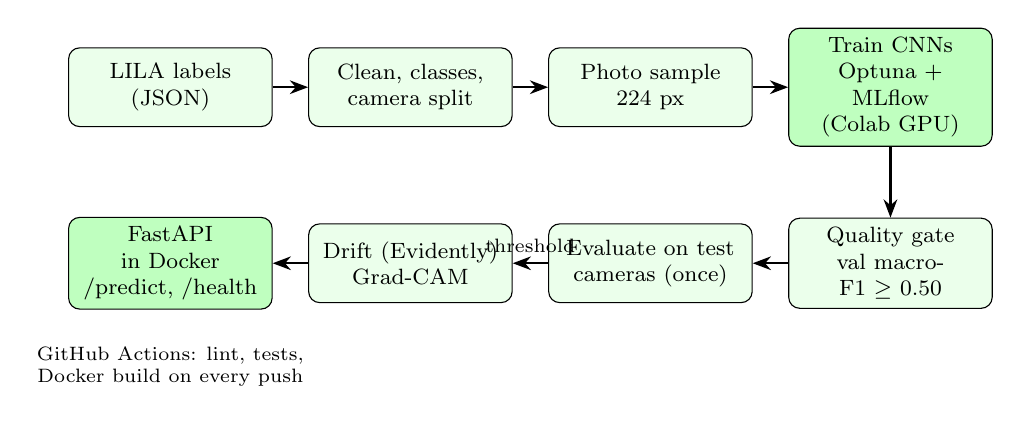
\begin{tikzpicture}[
  box/.style={draw, rounded corners, fill=green!8, align=center, font=\footnotesize,
              minimum height=1.0cm, text width=2.35cm},
  dark/.style={box, fill=green!25},
  arrow/.style={-{Stealth}, thick}]
\node[box] (labels) {LILA labels\\ (JSON)};
\node[box, right=0.45cm of labels] (clean) {Clean, classes,\\ camera split};
\node[box, right=0.45cm of clean] (photos) {Photo sample\\ 224 px};
\node[dark, right=0.45cm of photos] (train) {Train CNNs\\ Optuna + MLflow\\ (Colab GPU)};
\node[box, below=0.9cm of train] (gate) {Quality gate\\ val macro-F1 $\geq$ 0.50};
\node[box, left=0.45cm of gate] (eval) {Evaluate on test\\ cameras (once)};
\node[box, left=0.45cm of eval] (mon) {Drift (Evidently)\\ Grad-CAM};
\node[dark, left=0.45cm of mon] (api) {FastAPI in Docker\\ /predict, /health};
\draw[arrow] (labels) -- (clean);
\draw[arrow] (clean) -- (photos);
\draw[arrow] (photos) -- (train);
\draw[arrow] (train) -- (gate);
\draw[arrow] (gate) -- (eval);
\draw[arrow] (eval) -- node[above, font=\scriptsize]{threshold} (mon);
\draw[arrow] (mon) -- (api);
\node[below=0.35cm of api, font=\scriptsize, align=center] {GitHub Actions: lint, tests,\\ Docker build on every push};
\end{tikzpicture}
\caption{Architecture. Every box is a script in \texttt{src/camtrap/}; settings live in \texttt{configs/config.yaml}.}
\end{figure}

Only the photo download and training run on Google Colab, because they need Google's network and a
GPU; the notebook there only clones the repository and calls the same scripts. The final model
(26\,MB), its settings and the MLflow runs are committed, so the API runs without retraining.

% ---------------------------------------------------------------- 4
\section{Methods and technique justification}

\subsection{Models}
I compared four models of increasing power, so that each step has to earn its place:
\begin{enumerate}
\item \textbf{Dummy classifiers} (most frequent, stratified): the score of a model that ignores the photo.
\item \textbf{Logistic regression on pretrained features:} EfficientNetB0 \cite{tan2019} turns each photo
      into 1,280 numbers, and a balanced, regularised logistic regression classifies them. The strength
      $C$ was chosen by 5-fold cross-validation grouped by camera (\texttt{GroupKFold}), never by photo.
\item \textbf{CNN from scratch:} the Lab~7 design (four Conv--MaxPool blocks with 16 to 128 filters,
      a dense layer and dropout), to test whether a small network can learn this task from 5,700 photos.
\item \textbf{Fine-tuned EfficientNetB0:} the ImageNet network with a new 14-class output; the last layers
      may be unfrozen. EfficientNetB0 gives the best accuracy per parameter of the standard Keras
      backbones and stays small enough to serve on a CPU.
\end{enumerate}
Both CNNs use Adam, cross-entropy and balanced class weights, and are tuned with Optuna \cite{akiba2019}:
a TPE sampler with a fixed seed and a median pruner that stops weak trials after two epochs. Each trial
trains for 6 epochs and returns validation macro-F1; the best setting is retrained with early stopping on
validation loss. The search space covers learning rate (log scale), dropout, augmentation on/off and either
dense size (scratch) or the number of unfrozen layers (0, 20 or 50). Every trial is logged to MLflow.

\subsection{Metrics}
The main metric, fixed before training, is \textbf{macro-F1 on the validation cameras}. It weights the 14
classes equally, so a rare species counts as much as a common one. Accuracy was ruled out because
answering ``empty'' every time is 90.2\% accurate on the real validation bursts but has a macro-F1 of
only 0.068. ROC-AUC was not used as the headline because it looks optimistic on imbalanced data. Around
the main metric I report per-class precision and recall, the multi-class Brier score, a 95\% interval from a
bootstrap that resamples \emph{cameras} (photos from one camera are not independent), the gap between
validation and test, and day against night.

\subsection{Calibration and the review rule}
The service must decide which photos a person should check. An isotonic regression (Lab~3) maps the
model's confidence to the observed accuracy on the validation cameras. A photo is sent to review if its
calibrated confidence is below a threshold; the threshold is chosen on validation to minimise cost, with a
wrong label costing 5 times a review. The threshold is then applied unchanged to the test cameras.

\subsection{Explanation and monitoring}
Grad-CAM \cite{selvaraju2017} shows which parts of a photo drive the prediction. It is also used to test a
specific shortcut: the text strip with the date and time, which could reveal night animals or a camera.
Evidently compares the training and test cameras on brightness, contrast, colour, share of green, hour,
and the first five principal components of the image features (PCA fitted on training cameras, Lab~5).

\subsection{What I chose not to do}

\begin{table}[H]
\centering\small
\begin{tabularx}{\textwidth}{p{4.1cm}X}
\toprule
Alternative & Why it was ruled out \\
\midrule
Random or stratified split & Lets the model recognise the place: it scored 0.72 macro-F1 against 0.58
with a camera split (Section~5.1). \\
Accuracy, micro-F1, ROC-AUC as headline & Dominated by the majority class or optimistic under imbalance. \\
Two-stage model (empty filter, then species), as in the proposal & One 14-class model gives both answers in one call;
its empty filter keeps 91\% of animals. A second model would double training time on a limited GPU quota. Left as future work. \\
Focal loss (proposal) & Balanced sampling plus class weights already handle the imbalance; focal loss adds a hyperparameter and was not part of the course. \\
Animal crops from a detector (MegaDetector \cite{beery2019}) & Adds a second, external model to the pipeline and the API; Grad-CAM shows the model already looks at the animal in most photos. \\
Larger backbones (ResNet50, vision transformers) & Free Colab GPU time was the limit (the quota ran out after training); a 26\,MB model is also easier to serve in Docker on a CPU. \\
Gradient boosting or SVM on the features & The linear probe already reaches 0.59; the question is about sites, not about squeezing the probe. \\
Oversampling (SMOTE) & Not meaningful for images; the sample is balanced by design instead. \\
Grid search & Optuna's TPE with pruning reaches good settings in 10--12 trials. \\
Temperature scaling & Isotonic calibration was taught in Lab~3 and needs no extra training; the model turned out to be well calibrated anyway. \\
Clustering, LLMs, retrieval & Labels exist and the input is an image; these do not fit the task. \\
\bottomrule
\end{tabularx}
\caption{Alternatives considered and ruled out.}
\end{table}

Two further changes from the proposal: a CNN from scratch was added as a comparison (the proposal ruled
it out for compute reasons; it trains in minutes on a T4), and the planned simulated low-light and
blocked-view tests were replaced by the real day/night split, which tests the same weakness on real photos.
The optional extra test on a Kenyan site was not added in the time available, so the unseen-site test uses
held-out Serengeti cameras.

% ---------------------------------------------------------------- 5
\section{Results}

\subsection{Random split against camera split}
With the same logistic regression, 5-fold cross-validation on the training cameras gives a macro-F1 of
\textbf{0.719 with a random split} but \textbf{0.582 when whole cameras are held out}. A random split
would have overstated performance by about 0.14. The camera-split estimate turned out to be close to the
final test result, which supports using it.

\subsection{Model comparison}

\begin{table}[H]
\centering\small
\begin{tabular}{lcccc}
\toprule
Model & Val macro-F1 & Test macro-F1 & Test accuracy & Test Brier \\
\midrule
Dummy (always empty), all validation bursts & 0.068 & -- & -- & -- \\
Logistic regression on features & 0.560 & 0.586 & 0.596 & 0.521 \\
CNN from scratch (Optuna) & 0.132 & 0.148 & 0.171 & 0.904 \\
\textbf{EfficientNetB0 fine-tuned (Optuna)} & \textbf{0.586} & \textbf{0.598} & \textbf{0.610} & \textbf{0.507} \\
\bottomrule
\end{tabular}
\caption{Results. The final model was chosen on validation macro-F1 before the test cameras were scored.}
\end{table}

The fine-tuned EfficientNetB0 is the final model (learning rate $1.2\times10^{-4}$, last 20 layers unfrozen,
dropout 0.20, no augmentation; 7 epochs). It passed the quality gate. On the 25 unseen test cameras it reaches a
macro-F1 of \textbf{0.598 (95\% interval 0.533--0.633)}.

Three points need interpreting rather than just reporting. First, the \textbf{fine-tuned model beats the
linear probe by only 0.012}, inside the confidence interval. Optuna's parameter importance agrees:
learning rate and dropout explain almost all the variation between trials, while the number of unfrozen
layers and augmentation explain almost none (Figure~\ref{fig:optuna}). With about 450 photos per class,
most of the useful knowledge comes from ImageNet, and fine-tuning adds little.

Second, the \textbf{CNN from scratch failed in an informative way}. Its training accuracy rose to 48\%
while validation accuracy stayed below 20\% and validation loss rose from the second epoch
(Figure~\ref{fig:scratch}). With 117 training cameras, the easiest pattern to learn is the background of each
camera, not the animal, which is exactly the site effect this project is about \cite{beery2018}. It failed the quality gate.

\begin{figure}[H]
\centering
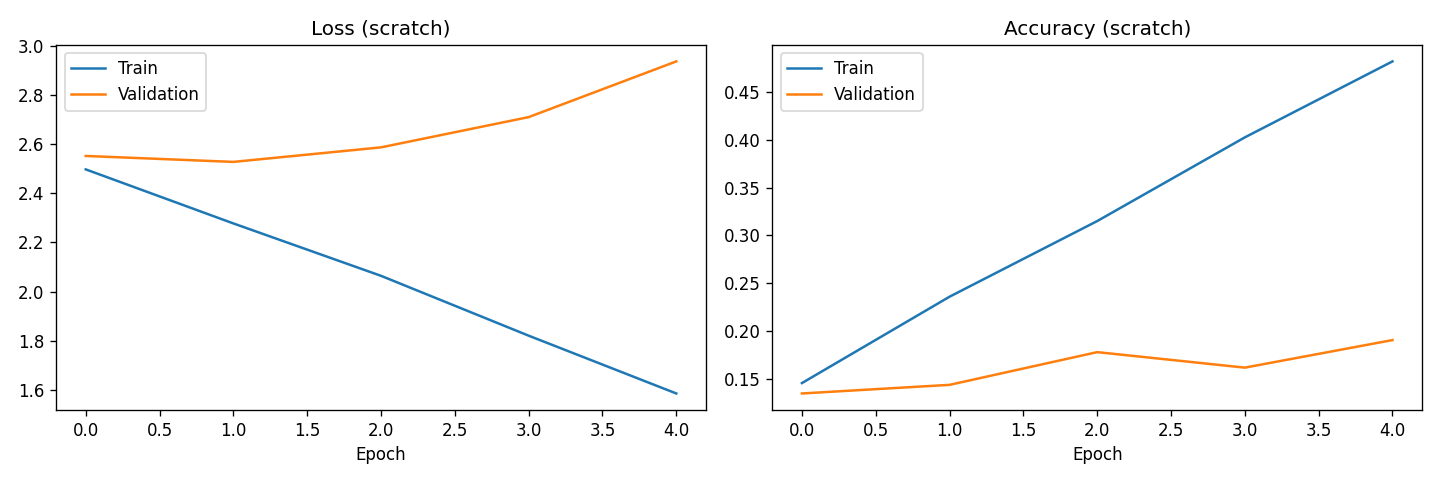
\includegraphics[width=0.85\textwidth]{training_scratch.png}
\caption{CNN from scratch: training improves, validation does not. The model memorises the training cameras.}
\label{fig:scratch}
\end{figure}

\begin{figure}[H]
\centering
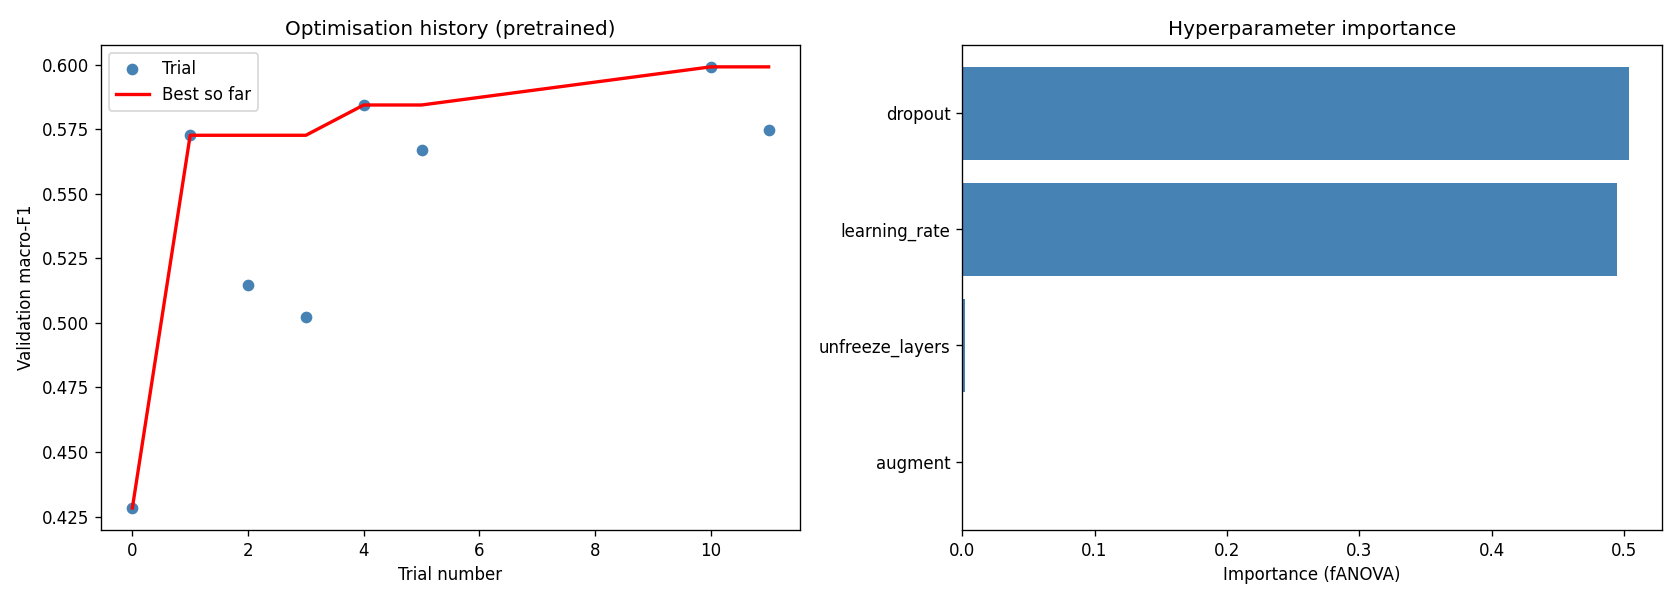
\includegraphics[width=0.85\textwidth]{optuna_pretrained.png}
\caption{Optuna study for EfficientNetB0: optimisation history (left) and parameter importance (right).}
\label{fig:optuna}
\end{figure}

Third, the \textbf{test score is not lower than validation} ($-0.012$ gap). The model does not lose
performance on a second set of unseen cameras, which is the main answer to the project question. It should
not be read as an improvement: the difference is well inside the interval.

\subsection{Per class, day and night}
Giraffe (F1 0.77), guineafowl, hartebeest and warthog (about 0.71) are easiest. The weakest classes are
\texttt{other} (0.24), which mixes many species, reedbuck (0.33, only 26 test photos) and \texttt{empty}
(0.45). The low precision of \texttt{empty} (0.36) means that some animals are called empty: as an empty
filter, the model keeps 91\% of the animals while removing 60\% of the empty photos.
Night photos are clearly harder: macro-F1 is \textbf{0.40 at night against 0.58 by day} (280 and 998 photos).

\begin{figure}[H]
\centering
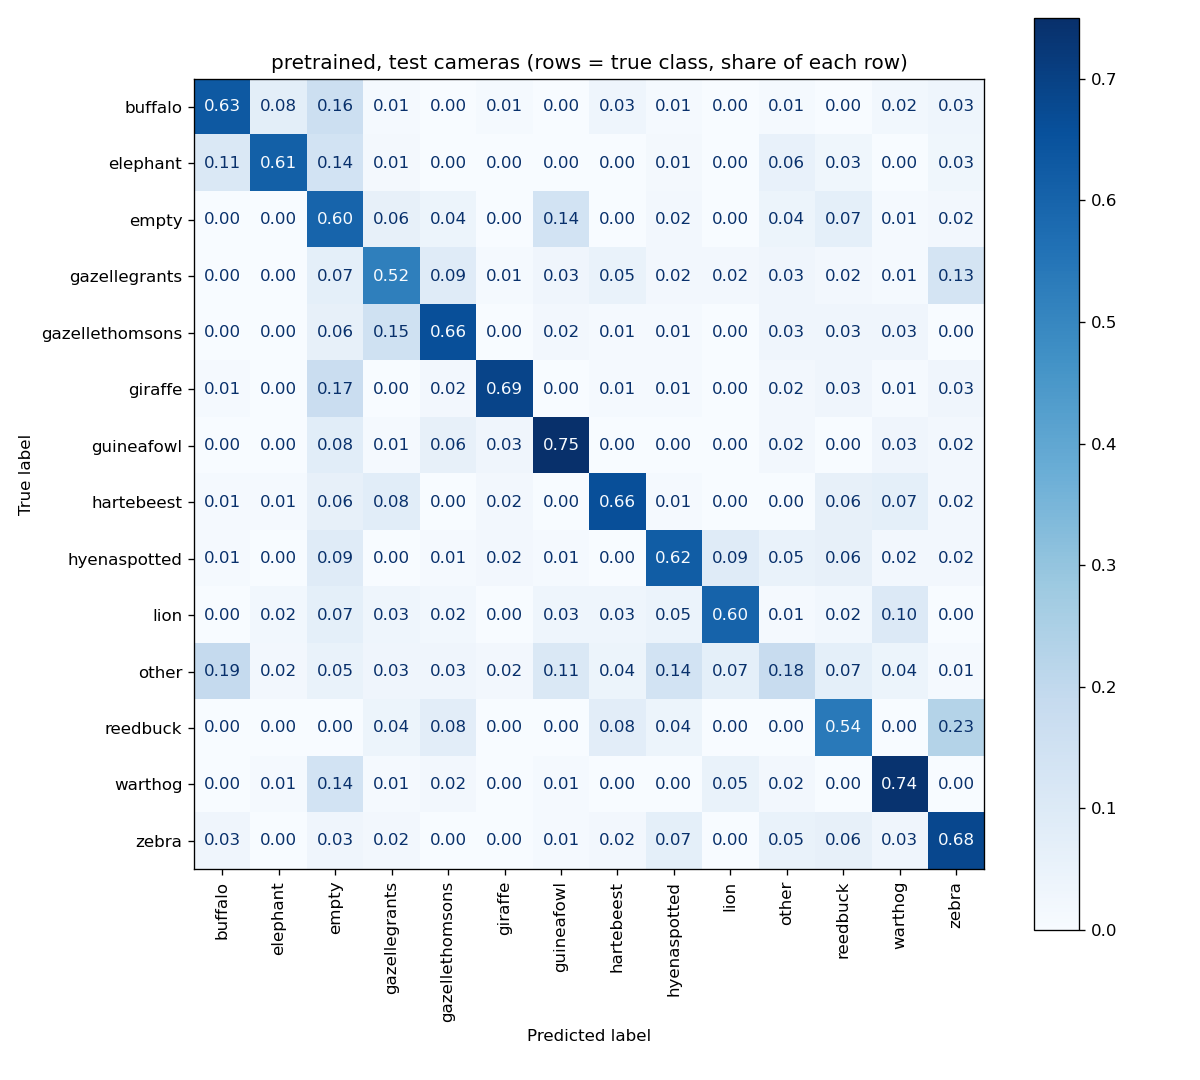
\includegraphics[width=0.62\textwidth]{test_confusion_matrix.png}
\caption{Confusion matrix on the test cameras (rows: true class, normalised).}
\end{figure}

\subsection{Calibration and human review}
The model's confidence was already well calibrated: the confidence Brier score is 0.159 before and after
isotonic calibration (Figure~\ref{fig:review}, left). The threshold chosen on validation (calibrated
confidence 0.865) sends \textbf{60\% of test photos to a person}, and the 40\% accepted automatically are
\textbf{92\% correct}. With a wrong label costing 5 times a review, this costs 76 units per 100 photos,
against 100 for checking everything and 195 for accepting everything.

\begin{figure}[H]
\centering
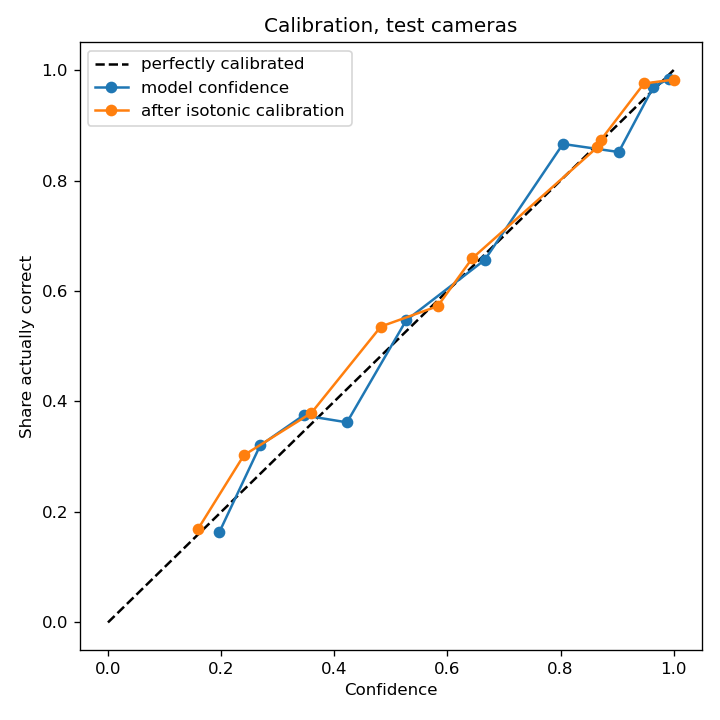
\includegraphics[width=0.36\textwidth]{test_calibration.png}\hfill
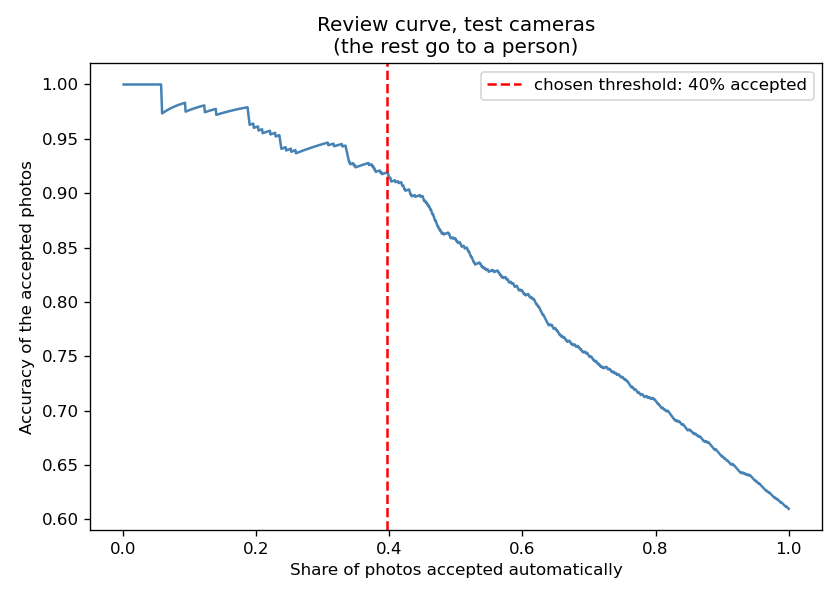
\includegraphics[width=0.6\textwidth]{test_review_curve.png}
\caption{Left: calibration on the test cameras. Right: accuracy of the photos accepted automatically
against the share accepted; the red line is the chosen threshold.}
\label{fig:review}
\end{figure}

\subsection{Where the model looks}
On correct answers the Grad-CAM heat sits on the animal (Figure~\ref{fig:gradcam}). The most confident
mistakes have three causes: animals so close that only a leg or belly is visible, small distant animals
called \texttt{empty}, and frames with several animals.

The date strip is \textbf{not} a shortcut. Only 2.1\% of the Grad-CAM heat falls on it, against 6.7\% if the
heat were spread evenly, and painting it grey on every test photo leaves macro-F1 unchanged (0.598 to
0.602). However, 16\% of individual answers change when the strip is painted, so the model is sensitive to
edits in that area even though it does not rely on it.

\begin{figure}[H]
\centering
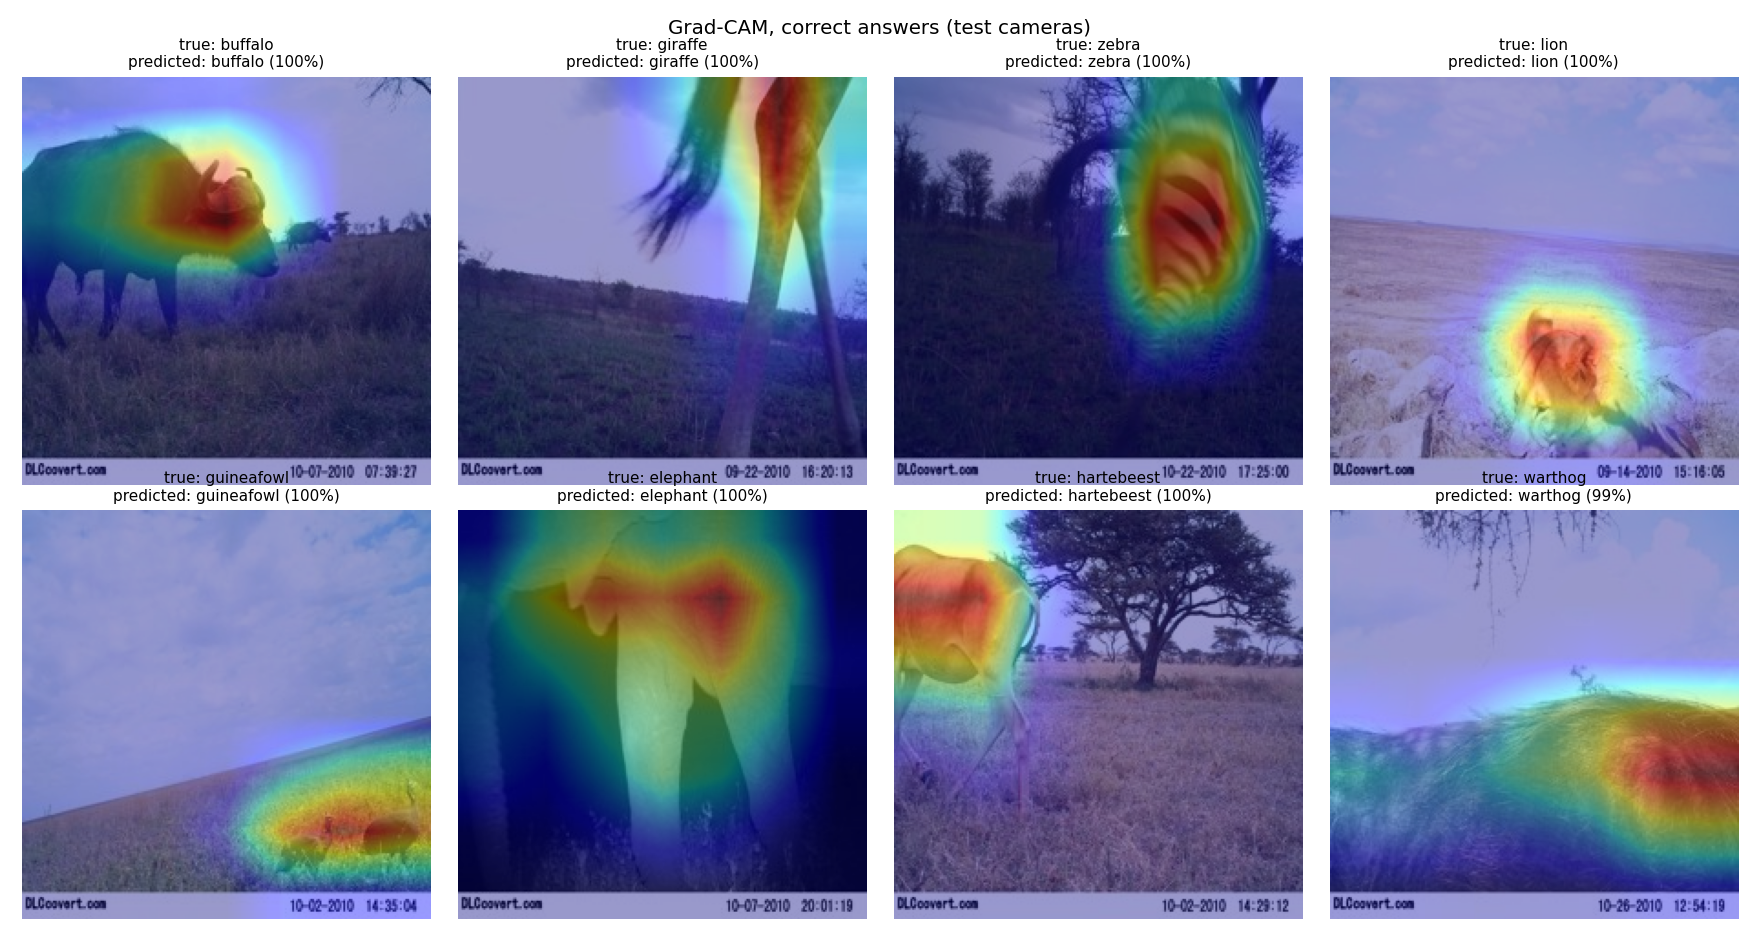
\includegraphics[width=\textwidth]{gradcam_correct.png}\\[4pt]
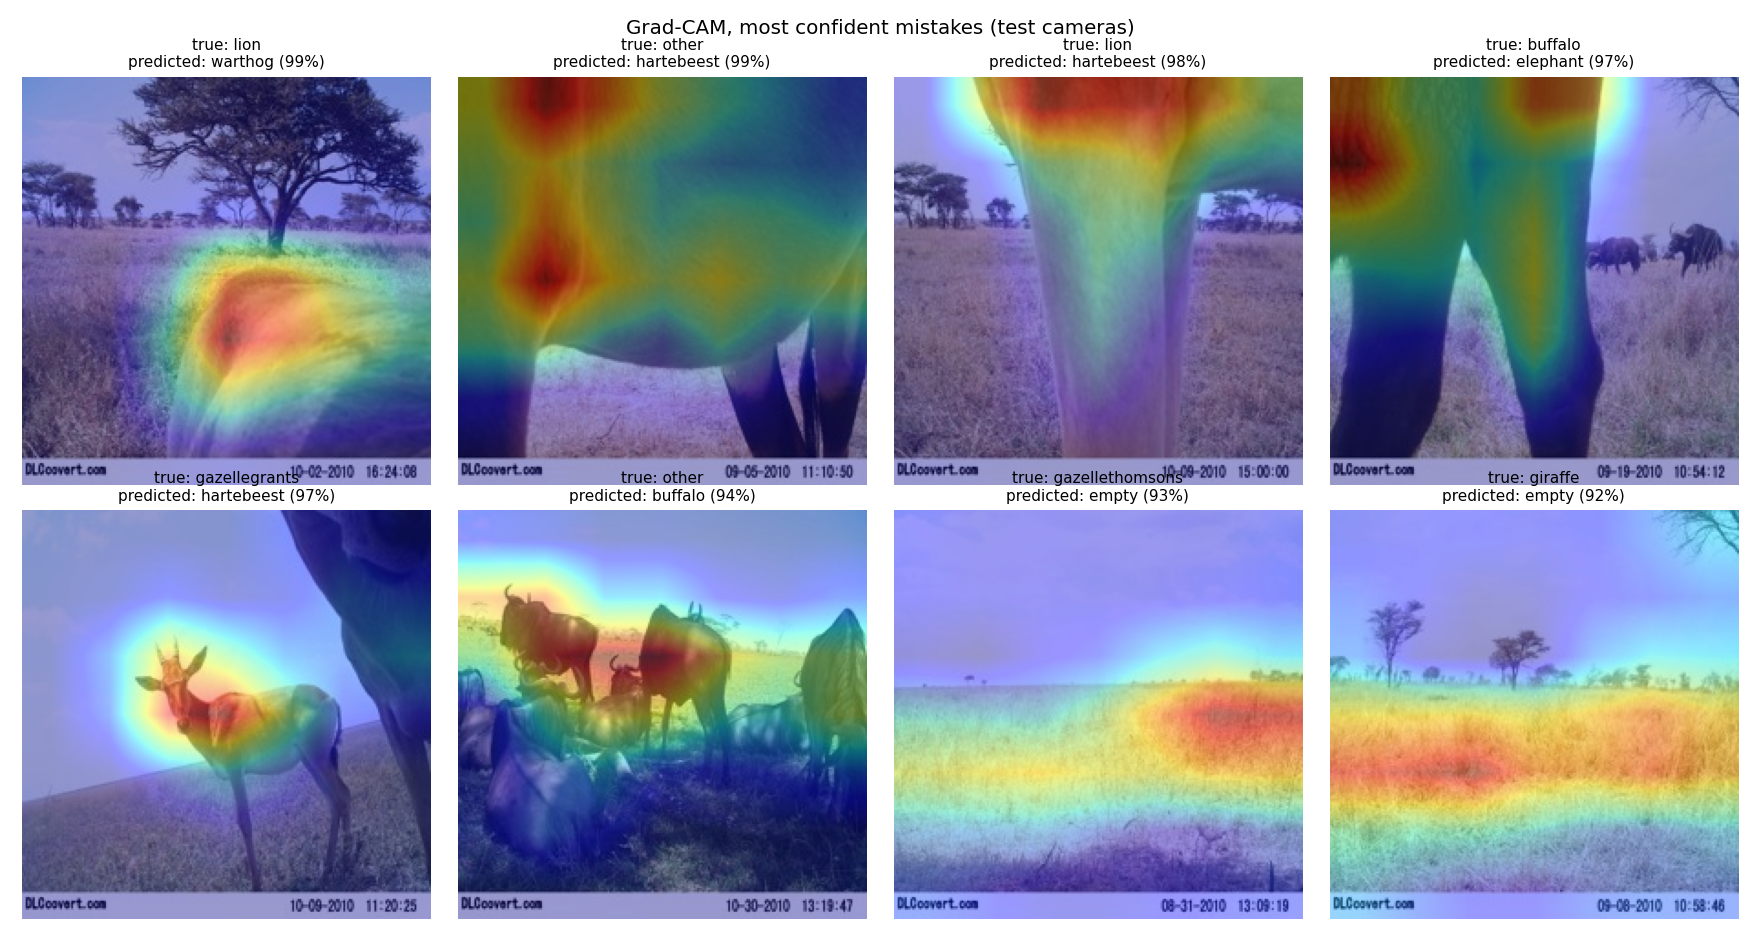
\includegraphics[width=\textwidth]{gradcam_wrong.png}
\caption{Grad-CAM on test cameras: correct answers (top) and the most confident mistakes (bottom).}
\label{fig:gradcam}
\end{figure}

\subsection{Drift between training and test cameras}
Evidently finds small drift: 4 of 10 columns pass its threshold (normalised Wasserstein distance $\geq 0.1$).
The share of green differs most (0.23), reflecting different vegetation; brightness, contrast, colour and
hour do not drift. In the PCA projection the test cameras sit inside the cloud of training cameras. New
cameras look different but not unfamiliar, which fits the stable test score. The five components keep only
26\% of the feature variance, so this check is coarse.

% ---------------------------------------------------------------- 6
\section{Deployment}
The model is served by a FastAPI service (\texttt{src/camtrap/serving/app.py}). \texttt{POST /predict}
takes a photo and returns the species, the raw and calibrated confidence, the top three answers and a
\texttt{needs\_review} flag; \texttt{GET /health} reports whether a model is loaded. The model is loaded
once at start-up and only if it passed the quality gate; the calibration and threshold come from the
evaluation, so the service flags photos exactly as in Section~5.4. A Dockerfile builds a small CPU image
(only the API's packages), and \texttt{docker compose up} starts the API together with an MLflow dashboard
of all training runs. Six pytest tests check the API with a stand-in model, and GitHub Actions lints the
code, runs the tests, builds the Docker image and checks \texttt{/health} on every push.

% ---------------------------------------------------------------- 7
\section{Limitations}
\begin{itemize}
\item \textbf{One season, one park.} All cameras are from Serengeti Season~1. Different seasons, parks or
      camera models may shift the data more than held-out cameras do.
\item \textbf{A balanced sample, not the real mix.} The test sample has at most 100 photos per class, so
      macro-F1 measures ability per class. On the real stream (83\% empty) accuracy and the precision of
      \texttt{empty} would be much higher, and the cost figures would change.
\item \textbf{Small and uneven test classes.} Reedbuck has 26 test photos and 25 test cameras give a wide
      interval (0.53--0.63); small differences between models are not significant.
\item \textbf{Night and close-ups} remain weak, and multi-animal bursts were removed, so the model never
      learned to handle them.
\item \textbf{Label noise.} Volunteer labels are per burst; one photo per burst may not show the animal.
      Imperfectly detected animals (MNAR) cannot be measured.
\item \textbf{Limited tuning.} 10--12 Optuna trials of 6 epochs each, on a free GPU quota.
\end{itemize}

% ---------------------------------------------------------------- 8
\section{Real-world relevance and conclusion}
For a conservation team the useful result is not the 0.60 macro-F1 but the workflow: the model can take
40\% of the photos off a reviewer's desk at 92\% accuracy and route the rest to people, at about three
quarters of the cost of checking everything, while keeping 91\% of animals when used as an empty filter.
The same pipeline can be pointed at a new park's metadata through the config file.

The project's main lessons are about evaluation. A random split would have reported 0.72 instead of 0.58;
a model trained from scratch would have memorised camera backgrounds; and a reported accuracy of 90\%
could describe a model that never sees an animal. Splitting by camera, measuring macro-F1 and checking
where the model looks showed what the model can actually do on a site it has never seen. Next steps are a
second season or park as a harder test, a dedicated empty filter, and more training data for night photos.

% ---------------------------------------------------------------- References
\begin{thebibliography}{9}\small
\bibitem{akiba2019} T.~Akiba, S.~Sano, T.~Yanase, T.~Ohta and M.~Koyama. Optuna: A next-generation
hyperparameter optimization framework. \emph{Proc.\ KDD}, 2019.
\bibitem{beery2018} S.~Beery, G.~Van Horn and P.~Perona. Recognition in terra incognita.
\emph{Proc.\ ECCV}, 2018.
\bibitem{beery2019} S.~Beery, D.~Morris and S.~Yang. Efficient pipeline for camera trap image review.
\emph{arXiv:1907.06772}, 2019.
\bibitem{norouzzadeh2018} M.~S.~Norouzzadeh, A.~Nguyen, M.~Kosmala, A.~Swanson, M.~S.~Palmer, C.~Packer
and J.~Clune. Automatically identifying, counting, and describing wild animals in camera-trap images with
deep learning. \emph{PNAS}, 115(25):E5716--E5725, 2018.
\bibitem{selvaraju2017} R.~R.~Selvaraju, M.~Cogswell, A.~Das, R.~Vedantam, D.~Parikh and D.~Batra.
Grad-CAM: Visual explanations from deep networks via gradient-based localization. \emph{Proc.\ ICCV}, 2017.
\bibitem{swanson2015} A.~Swanson, M.~Kosmala, C.~Lintott, R.~Simpson, A.~Smith and C.~Packer. Snapshot
Serengeti, high-frequency annotated camera trap images of 40 mammalian species in an African savanna.
\emph{Scientific Data}, 2:150026, 2015.
\bibitem{tan2019} M.~Tan and Q.~V.~Le. EfficientNet: Rethinking model scaling for convolutional neural
networks. \emph{Proc.\ ICML}, 2019.
\end{thebibliography}

\end{document}
